\section{Methodology}
\label{sec:methodology}

\begin{figure*}[!t]
    \centering
    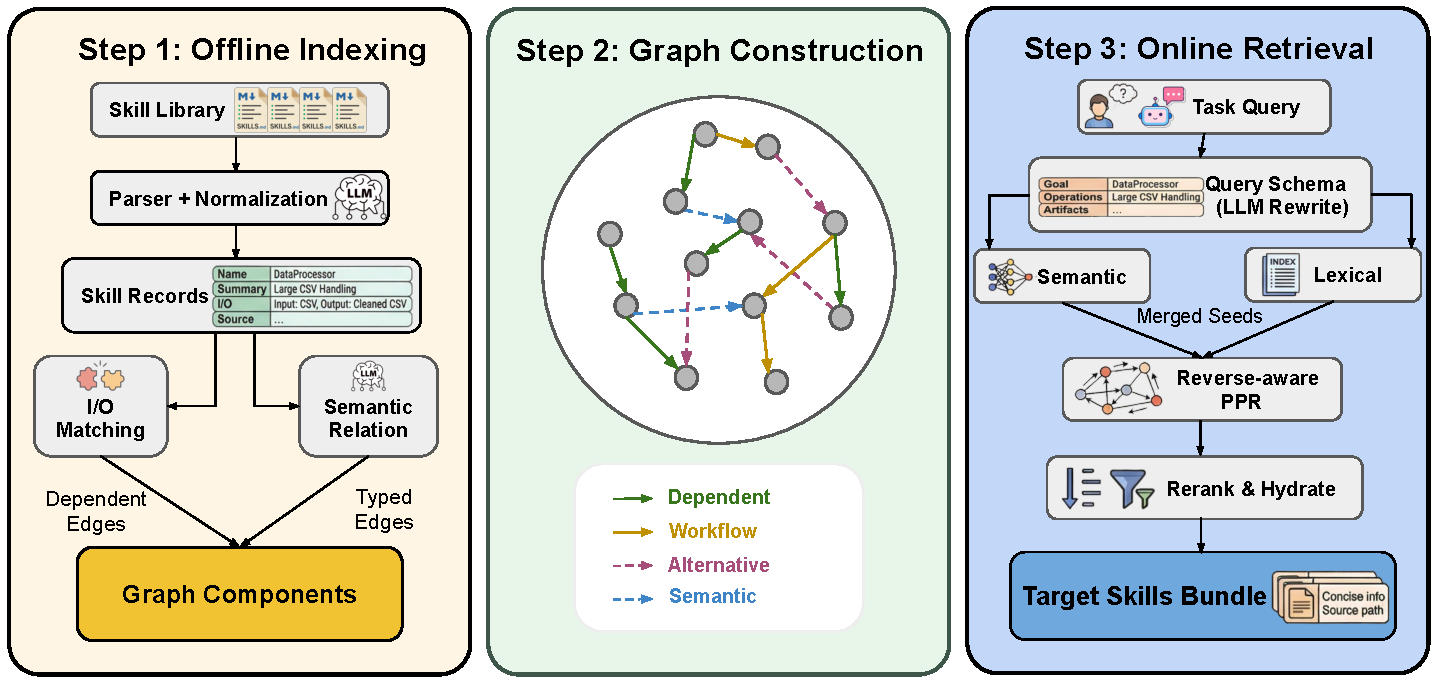
\includegraphics[width=1\linewidth]{assests/arch.pdf}
    \caption{Overview of Graph of Skills (GoS). \textbf{Left:} offline indexing converts local \skillpackages{} into normalized skill records and typed edges. Dependency edges are induced from I/O compatibility, while workflow, semantic, and alternative relations are added through sparse validation. \textbf{Center:} the typed directed skill graph is the retrieval substrate; edge labels denote dependency, workflow, semantic, and alternative relations. \textbf{Right:} online retrieval maps a task query to a compact query schema, forms merged seeds from semantic and lexical retrieval, applies reverse-aware Personalized PageRank, and returns a budgeted execution bundle after reranking and hydration.}
    \label{fig:gos_arch_horizontal}
\end{figure*}

GoS is an inference-time retrieval layer for large local skill libraries. It constructs a typed graph offline from local \skillpackages{} and, at query time, returns a compact execution bundle that is relevant to the task and more likely than flat retrieval to include the prerequisites required for successful execution.

\subsection{Problem Setup}
Let $\mathcal{C} = \{d_1, \dots, d_m\}$ denote a local corpus of \skillpackages{}. Each package contains a primary specification document together with optional scripts, references, and auxiliary assets. GoS converts $\mathcal{C}$ into a typed directed graph
\begin{equation}
    G = (V, E, w, \phi),
\end{equation}


where each node $v \in V$ is a normalized executable skill record, each edge $e \in E$ connects two skills, $w(e) > 0$ is an edge weight, and $\phi(e) \in \mathcal{R}$ assigns an edge type from the relation set
\begin{equation}
\mathcal{R} = \{\mathrm{dep}, \mathrm{wf}, \mathrm{sem}, \mathrm{alt}\}.
\end{equation}

Given a task query $q$ and a context budget $\tau$, the retrieval problem is to return a bundle $B(q) \subseteq V$ that is simultaneously relevant, execution-complete when possible, and compact. We view this as a budgeted selection problem,
% \begin{equation}
% \begin{aligned}
% \max_{B \subseteq V} \; & \sum_{v \in B} \operatorname{rel}(v, q) \\
% & + \beta \!\!\!\!\sum_{(u,v) \in E_{\mathrm{dep}}} \!\!\!\!\mathbb{I}[u \in B \wedge v \in B] \\
% & \text{s.t.} \; \operatorname{cost}(B) \le \tau,
% \end{aligned}
% \label{eq:objective}
% \end{equation}
\begin{equation}
\begin{aligned}
\max_{B \subseteq V} \; & \sum_{v \in B} \operatorname{rel}(v, q) + \beta \!\!\!\!\sum_{(u,v) \in E_{\mathrm{dep}}} \!\!\!\!\mathbb{I}[u \in B \wedge v \in B] \\
& \text{s.t.} \quad \operatorname{cost}(B) \le \tau
\end{aligned}
\label{eq:objective}
\end{equation}
where the first term favors query relevance, the second rewards dependency-complete bundles, and $\operatorname{cost}(B)$ measures the prompt budget consumed by the hydrated bundle. Equation~\eqref{eq:objective} is not solved exactly. Instead, GoS approximates this objective through three stages: hybrid seed retrieval, reverse-aware graph diffusion, and budgeted reranking plus hydration.

\subsection{Offline Graph Construction}
\noindent\textbf{Skill Normalization.}
Each \skillpackage{} is parsed into a normalized skill record containing a canonical name, capability summary, I/O fields, domain tags, tooling, entrypoints, compatibility notes, and a stable local source path. This normalization step is primarily deterministic: the system extracts executable fields whenever possible and uses a lightweight LLM pass only to recover retrieval-critical semantic fields when package documentation is incomplete. The goal is to convert each local skill into a retrieval unit that an agent can directly consume at inference time.

\noindent\textbf{Typed Relation Induction.}
GoS uses four edge types. \emph{Dependency} edges represent executable prerequisites and form the primary structural relation in the graph. A dependency edge $v_i \rightarrow v_j$ is added \emph{deterministically} whenever the I/O schemas of $v_i$ and $v_j$ overlap above a fixed threshold, so that $v_i$ can plausibly provide an artifact consumed by $v_j$; no LLM call is involved. \emph{Workflow} edges capture common multi-step pipelines, \emph{semantic} edges connect near-duplicate or topically adjacent skills, and \emph{alternative} edges link interchangeable strategies for the same subproblem.

Rather than performing unconstrained all-pairs relation inference, GoS constructs the three non-dependency edge types through sparse LLM validation. For each node, it first forms a small candidate pool using lexical similarity, semantic neighbors, and I/O-based expansion, and only the top-$k$ candidates per node are submitted to a constrained validator prompt (default $k{=}8$). Total LLM validation calls therefore scale as $\mathcal{O}(N k)$ rather than $\mathcal{O}(N^2)$, and incremental indexing further reduces this to $\mathcal{O}(|V_{\mathrm{new}}|\,N)$. This keeps graph construction tractable while anchoring the resulting graph in executable structure rather than metadata proximity alone.

\subsection{Online Structural Retrieval}
\noindent\textbf{Query Representation and Hybrid Seeding.}
Dense retrieval~\citep{karpukhin2020dense} is often effective at finding the visible top-level skill but weak at recovering semantically subtle prerequisites. Lexical retrieval in the probabilistic ranking tradition~\citep{robertson2009probabilistic} is robust for concrete artifacts and filenames, but brittle under paraphrase. GoS therefore combines the two signals at the seeding stage.

At retrieval time, the raw query is mapped to a lightweight retrieval schema containing the task goal, salient operations, referenced artifacts, and normalized keywords. This schema can be produced by an optional LLM rewrite, following the general intuition of rewrite-then-retrieve pipelines~\citep{ma2023query}; when rewriting is unavailable or disabled, GoS falls back to deterministic lexical normalization. GoS then computes a semantic seed score $s_i^{\mathrm{sem}}(q)$ and a lexical seed score $s_i^{\mathrm{lex}}(q)$ for each candidate skill $v_i$, and merges them as
\begin{equation}
 z_i(q) = \eta \, s_i^{\mathrm{sem}}(q) + (1-\eta) \, s_i^{\mathrm{lex}}(q),
 \label{eq:seed}
\end{equation}
where $\eta \in [0,1]$ controls the semantic--lexical tradeoff. The initial seed distribution is obtained by normalizing the merged scores over the candidate pool,
\begin{equation}
\mathbf{p}_i = \frac{z_i(q)}{\sum_j z_j(q)}.
\end{equation}

\noindent\textbf{Reverse-Aware Typed Diffusion.}
Let $A_r$ denote the weighted adjacency matrix for relation type $r \in \mathcal{R}$. To let retrieval move from a matched high-level skill toward likely prerequisites, GoS uses both forward and reverse transitions. For each relation type, we define a row-normalized forward operator $T_r^{\rightarrow}$ and a row-normalized reverse operator $T_r^{\leftarrow}$ obtained from $A_r$ and $A_r^{\top}$, respectively. GoS then forms the unified transition operator
\begin{equation}
T = \operatorname{RowNorm}\!\left( \sum_{r \in \mathcal{R}} \lambda_r \left(T_r^{\rightarrow} + \gamma_r T_r^{\leftarrow}\right) \right),
\label{eq:transition}
\end{equation}
where $\lambda_r \ge 0$ and $\sum_r \lambda_r = 1$ weight relation types, and $\gamma_r \ge 0$ controls how strongly reverse traversal is allowed for each type. In practice, reverse edges are inserted directly into the transition matrix with type-specific weights (largest for dependency, smallest for alternative; concrete values in Appendix~\ref{tab:appendix_relation_weights}), and the matrix is row-normalized before diffusion.

The core retrieval step is a reverse-aware Personalized PageRank-style diffusion over this operator~\citep{page1999pagerank, jeh2003scaling, 10471277}:
\begin{equation}
\mathbf{s}^{(\ell+1)} = \alpha \, \mathbf{p} + (1-\alpha) T^{\top} \mathbf{s}^{(\ell)},
\label{eq:ppr}
\end{equation}
where $\alpha \in (0,1)$ is the restart parameter. Relative to flat top-$k$ retrieval, relevance is not assigned only to individually matched skills; it is propagated across a local executable neighborhood. In particular, once a high-level solver is retrieved as a seed, upstream parser, setup, or preprocessing skills can still accumulate score through reverse dependency paths even when they are not themselves strong semantic matches to the original query.

\noindent\textbf{Budgeted Reranking and Hydration.}
The diffusion score alone is insufficient, because the final output must be compact and directly usable by an agent. GoS therefore reranks candidate skills by combining graph score with field-level query evidence:
\begin{equation}
\rho_i(q) = \mathbf{s}_i^{\star} + \mu \, m_i(q),
\label{eq:rerank}
\end{equation}
where $\mathbf{s}_i^{\star}$ is the converged diffusion score, $m_i(q)$ aggregates direct matches between the query and skill fields such as name, capability summary, artifacts, and entrypoints, and $\mu$ controls how much local grounding is preserved after graph expansion.

Candidates are then hydrated in descending order of $\rho_i(q)$ under both per-skill and global context budgets. Here, \emph{hydration} denotes materializing a selected skill into an agent-consumable payload that includes a stable source path together with concise capability text and the most relevant execution notes. The final output is therefore a bounded execution bundle designed to maximize executable coverage within the prompt budget.


% GoS' central design choice is to cast retrieval as a structured bundle-selection problem: semantic and lexical matching identify promising entry points, graph diffusion recovers missing prerequisites, and budgeted hydration enforces compactness. This combination allows GoS to improve task reward while preserving the efficiency benefits of retrieval.
